%% 
%% Copyright 2007-2025 Elsevier Ltd
%% 
%% This file is part of the 'Elsarticle Bundle'.
%% ---------------------------------------------
%% 
%% It may be distributed under the conditions of the LaTeX Project Public
%% License, either version 1.3 of this license or (at your option) any
%% later version.  The latest version of this license is in
%%    http://www.latex-project.org/lppl.txt
%% and version 1.3 or later is part of all distributions of LaTeX
%% version 1999/12/01 or later.
%% 
%% The list of all files belonging to the 'Elsarticle Bundle' is
%% given in the file `manifest.txt'.
%% 
%% Template article for Elsevier's document class `elsarticle'
%% with numbered style bibliographic references
%% SP 2008/03/01
%% $Id: elsarticle-template-num.tex 272 2025-01-09 17:36:26Z rishi $
%%
%%\documentclass[preprint,12pt]{elsarticle}

%% Use the option review to obtain double line spacing
\documentclass[preprint,12pt,3p]{elsarticle}
%%if you are using elsarticle.cls, do not use it with options
%%    \documentclass[authoryear]{elsarticle}
%% and the style
%% \bibliographystyle{elsarticle-num}
%% https://tex.stackexchange.com/questions/54480/package-natbib-error-bibliography-not-compatible-with-author-year-citations

%% Use the options 1p,twocolumn; 3p; 3p,twocolumn; 5p; or 5p,twocolumn
%% for a journal layout:
%% \documentclass[final,1p,times]{elsarticle}
%% \documentclass[final,1p,times,twocolumn]{elsarticle}
%% \documentclass[final,3p,times]{elsarticle}
%% \documentclass[final,3p,times,twocolumn]{elsarticle}
%% \documentclass[final,5p,times]{elsarticle}
%% \documentclass[final,5p,times,twocolumn]{elsarticle}
%% https://tex.stackexchange.com/questions/261864/how-do-i-determine-the-attribute-of-elsarticle-document

\usepackage{threeparttable}
\usepackage{url}
\usepackage{multirow}
\usepackage{tabularx}
\usepackage{makecell}
\usepackage{placeins}
%\usepackage{tikz}
%\usetikzlibrary{calc}
\usepackage[figuresleft]{rotating}
\usepackage{longtable, lscape, booktabs, array}
%usepackage[nodisplayskipstretch]{setspace}\setstretch{1.5}

\usepackage{amsmath}

\DeclareMathOperator{\logit}{\textrm{logit}}

%% For including figures, graphicx.sty has been loaded in
%% elsarticle.cls. If you prefer to use the old commands
%% please give \usepackage{epsfig}

%% The amssymb package provides various useful mathematical symbols
\usepackage{amssymb}
%% The amsmath package provides various useful equation environments.
\usepackage{amsmath}
%% The amsthm package provides extended theorem environments
%% \usepackage{amsthm}

%% The lineno packages adds line numbers. Start line numbering with
%% \begin{linenumbers}, end it with \end{linenumbers}. Or switch it on
%% for the whole article with \linenumbers.
\usepackage[mathlines, switch, columnwise]{lineno}


\journal{Computational and Structural Biotechnology Reports}

\begin{document}

\begin{frontmatter}

%% Title, authors and addresses

%% use the tnoteref command within \title for footnotes;
%% use the tnotetext command for theassociated footnote;
%% use the fnref command within \author or \affiliation for footnotes;
%% use the fntext command for theassociated footnote;
%% use the corref command within \author for corresponding author footnotes;
%% use the cortext command for theassociated footnote;
%% use the ead command for the email address,
%% and the form \ead[url] for the home page:
\title{Detection of Epistatic Interactions in High-Dimensional Genomic Data Using Random Forests}
  
\author[1]{Hawlader A. Al-Mamun\corref{cor1}\fnref{fn1}}
\ead{halmamun@intergrain.com}
\author[4]{Rob Dunne} %% Author name
\author[5]{Ross L. Tellam}
\author[1]{Klara Verbyla, \fnref{fn2}}

\cortext[cor1]{Corresponding author}


\affiliation[1]{organization={Agriculture \& Food, CSIRO},%Department and Organization
  addressline={2 - 40 Clunies Ross Street}, 
  city={Acton},
  postcode={2601}, 
  state={ACT},
  country={Australia}}


% \affiliation{organization={InterGrain Pty Ltd.},
%   addressline={19 Ambitious Link}, 
%   city={Bibra Lake},
%   postcode={6163}, 
%   state={WA},
%   country={Australia}}
% and
% \affiliation{organization={School of Biological Sciences},%Department and Organization
%   addressline={The University of Western Australia}, 
%   city={Crawley},
%   postcode={6009}, 
%   state={WA},
%   country={Australia}}

\fntext[fn1]{Currently at InterGrain Pty Ltd, 19 Ambitious Link, Bibra Lake, 6163, WA and
  School of Biological Sciences, The University of Western Australia, Crawley, 6009, WA Australia}

\affiliation[4]{organization={Data61, CSIRO},
  addressline={13 Garden Street}, 
  city={Eveleigh},
  postcode={2015}, 
  state={NSW},
  country={Australia}}

\affiliation[5]{organization={CSIRO Agriculture and Food},%Department and Organization
  addressline={306 Carmody Rd}, 
  city={St Lucia},
  postcode={4067}, 
  state={QLD},
  country={Australia}}


% \affiliation[6]{organization={The Center for Aquaculture Technologies},%Department and Organization
%   addressline={8445 Camino Santa Fe, Suite 104}, 
%   city={San Diego},
%   postcode={92121}, 
%   state={California},
%   country={USA}}
\fntext[fn2]{Currently at The Center for Aquaculture Technologies, 8445 Camino Santa Fe, Suite 104, San Diego, 92121,
  California, USA}


%% Abstract
\begin{abstract}
Epistatic interactions can play an important role in the genetic mechanisms that control phenotypic
  variation. However, identifying these interactions in high dimensional genomic data can be very challenging due to the
  large computational burden induced by the high volume of combinatorial tests that have to be performed to explore the
  entire search space.  Random Forests Decision Trees are widely used in a variety of disciplines and are often said to
  detect interactions.  However, Random Forests models do not explicitly detect variable interactions. Most Random
  Forests based methods that claim to detect interactions rely on different forms of variable importance measures that
  suffer when the interacting variables have very small or no marginal effects. The proposed Random Forests based method
  detects interactions using a two-stage approach and is computationally efficient. The approach is demonstrated and
  validated through its application on several simulated datasets representing different data structures with respect to
  genomic data and trait heritabilities. The method is also applied to two high dimensional genomics data sets to
  validate the approach. In both cases, the method results were used to identify several genes closely positioned to the
  interacting markers that showed strong biological potential for contributing to the genetic control for the respective
  traits tested.
\end{abstract}



%%Research highlights
\begin{highlights}
\item The method detects epistatic interactions in high dimensional genomic data.
\item Computationally efective and produces reliable results in the case of simulated and interpretable results in several real-world
  data sets
\end{highlights}



%% Keywords
\begin{keyword}
Epistatic interactions \sep  Random Forests \sep SNP data
\end{keyword}

\end{frontmatter}


\linenumbers
\section{Introduction}
Many phenotypes and disease traits in human, animals and plants are complex and involve many genes and their
interactions.  Quantitative traits such as human height or yeast growth are influenced by many genetic variants each
typically of small effect size.  Numerous genetic variants have been reported in genome-wide association studies (GWAS)
and quantitative trait loci (QTL) studies that are associated with various quantitative traits in different
species. However, for each trait, the reported variants cumulatively can explain only a portion of the total
heritability of the trait.  This phenomenon of unexplained heritability is termed ``missing heritability''
\cite[]{Maher2008}, which is partly due to not considering the genetic variant interactions (epistasis) between the
genetic markers \cite[]{Zuk.et.al.2012}.

Epistasis occurs when there is any non-additive interaction relationship between two or more genes in their combined
effects on a phenotype. It can be potentially identified when the effects of two or more genetic markers associated with
a trait differ from the sum of the individual marker effects. Understanding epistasis is important because it can help
explain the functional mechanisms of the genes that together contribute to disease or trait expression and enable more
targeted and nuanced interventions to be developed. For example, being able to estimate the effect of non-additive
interactions could potentially be exploited to improve the genetic predictions \cite[]{Ansarifar.et.al.2020} for
economically important traits such as wheat yield or carcass weight of cattle.

The most direct approach to detect epistatic interactions is to use linear models (LM) to evaluate all pair-wise loci
combinations to test for non-additive interactions associated with a complex trait \cite[]{Zhang.et.al.2008}. This type
of exhaustive search is only feasible when the number of candidate markers is relatively small or the computational
power available is extreme. However, as the number of markers in a dataset grows, this approach suffers from the
computational burden induced by the combinatorial number of tests that have to be performed. For example, The Welcome
Trust Case Control studies \cite[]{burtonGenomewideAssociationStudy2007brief} had 17,000 individuals (2,000 cases for
each of seven diseases and 3,000 combined controls) genotyped with the GeneChip 500K Mapping Array Set (Affymetrix
chip), which interrogated 500,568 SNPs. Thus, more than $1.25\times 10^{13}$ pairwise tests would need to be performed, which is
not computationally feasible using standard equipment. Moreover, recent technological advancements and reduced costs
have led to experimental designs utilising more than 1 million variants and markers for hundreds of individuals,
which massively confound the ability to identify interacting pairs of SNPs \cite[]{Ha.et.al2014,
  Gholami.et.el2014,1000GenomeProject.2015.brief,utah.edu}. Consequently, two step-based methods have been proposed to
detect epistatic interactions from genomic data, where in the first step markers were pre-selected or weighted and then
in the second step interaction testing was performed only on the reduced set of markers. The preselection can be
performed based on statistical tests (e.g., GWAS \cite[]{Pecanka.et.al.2017}) or machine learning methods with feature
selection \cite[]{Jiang.et.al.2009, Meng.et.al.2007}.




Random Forests (RF) algorithms are an ensemble learning method first proposed by Leo Breiman \cite[]{Breiman2001}. Ensemble
learning combines multiple learning algorithms/models to improve prediction or classification performance beyond what
could be obtained from the constituent models. In Random Forests, \textit{m} random samples (with replacement) are
selected by bootstrap sampling. Then multiple decision trees are created based on the bootstrap samples. To break down
the correlation between features, only a random subset of features is considered at any node of the tree building
process. For classification problems, the class of the validation data is predicted based on majority voting and for the
regression problem, the model outputs the mean of the individual tree's prediction. There are two main parameters in the
implementation of the Random Forests algorithm, namely the number of decision trees (num.trees) and the number of
randomly selected features (\texttt{mtry}) from which the best feature for splitting is selected at any given node.

Random Forests models are widely used \cite[]{lundbergConsistentIndividualizedFeature2019} in a variety of
disciplines. The attraction of the model is based on several attributes, namely:
\begin{itemize} 
\item a high degree of accuracy;
\item a resistance to overfitting, including in the presence of large numbers of redundant variables; 
\item the provision of an out-of-bag error measure; 
\item the provision of a variable ranking at little extra computational cost.
\end{itemize}
 
In addition it is clear that Random Forests can perform well with correlated and interacting variables, at least in the
sense that the fitted model performs well \cite[]{Ziegler.et.al.2007}. However, most of the Random Forests based
approaches are either based on single variable importance \cite[]{Jiang.et.al.2009, yoshidaSNPInterForestNewMethod2011}
or based on pairwise variable importance \cite[]{Ziegler.et.al.2007}. The Random Forests-based approaches for identifying
interactions based on variable importance measurements cannot distinguish whether a discovered interaction is a true
interaction or simply two variables with strong marginal effects. Additionally, if the interacting variables have small
marginal effects, they will not appear near the top of the variable importance list. This means that detecting
interactions based on variable importance can be problematic. It is also heavily dependent on extensive permutation
tests.  \cite{schmalohrDetectionEpistaticInteractions2018} notes that there is a lack of accurate methods for the
detection of interactions between genomic loci that affect QTLs but that several studies have shown that RF outperforms
other QTL mapping methods at identifying QTL and discrete trait associations. They provided benchmarks on simulated and
real yeast cross data indicating that the RF-based methods outperform other commonly used approaches for detecting
epistasis.

To overcome the challenge of a large number of pairwise SNP interaction tests, we proposed an effective two-step process
based on our observations from using a Random Forests approach. Using simulation data, we observed that \textit{``if two SNPs are
interacting, they appear as parent-child nodes in a decision tree of a Random Forests more frequently than if they are
not interacting''}.

This new method and the validation results obtained using simulated data are presented in this manuscript. In
addition, the results from the use of the method using two real datasets are discussed.


\section{Methods}

The proposed method is described in Figure \ref{figure:RF_Method}. First, a Random Forests model is created using all
available genomic data. For both the simulated and real data examples, the R package ranger
\cite[]{Wright.and.Ziegler.2017} was used with the parameters \texttt{num.tree} = 1000 and \texttt{mtry} = \#SNPs/3.
%Once the Random Forests model is built, the number of times each pair of markers was found as parent-child nodes in all
%the decision trees were recorded,
Working from the Random Forests output, we can form a $p \times p$ matrix of values such that the $\{i,j\}^{th}$ entry is the count of the
number of times variable $v_i$ is followed by variable $v_j$.  If we sum the upper and lower triangular matrices and set the diagonal to 0,
we form the interaction vector, of length $\frac {p(p-1)} 2 = {p \choose 2}$.  This is likely to be large and contain a large number of
zeros ($4 \times 10^9$ entries and 0.999 zero in the rheumatoid example, section \ref{subsection: rheumatoid}).

\subsection{The Null Distribution}

Efron's Empirical Bayes procedure \cite[]{efronLargeScaleInferenceEmpirical2010} is now widely used to determine levels of significance in
high throughput genomics data analysis.  These data sets led to the use of large numbers of parallel tests to determine the significant
variables and the use of multiple testing corrections \cite{limma.2015}.  Efron suggests that instead of assuming a distribution, such as
the $t$, the better approach is to use the large number of variables to model the null distribution, and then do significance testing.


Applying the insights of Efron's work to this problem we start with the assumption that:
\begin{itemize}
\item most of the counts values come from a null distribution, that is a distribution of interaction
  counts that we would observe if there was no signal in the data and these counts were random values from some null distribution;
\item there is a smaller set of interactions that reflect the underlying biological processes. These are drawn from a
  different distribution to the null counts.
\end{itemize}

We model the data as 
\[
f (j ) = \pi_0 f_0 (j ) + (1 - \pi_0 )f_1 (j )
\]
where $j$ is the count data, $f_0$ is the null distribution and $f_1$ is some contaminating distribution of the
non-null counts. Following \cite{Gauran.et.al.2018} we could make the additional assumption that there is some integer $C$ such that
\begin{equation}
  f(j ) = \pi_0 f_0 (j ) \textrm{ for } j \leq C.
\label{eqn:C}  
\end{equation}
So we only have the null distribution for counts less than $C.$ 

As we have count data we model the null distribution $f_0$ as a Poisson or  generalized Poisson ($g$, with parameters
$\lambda$ and $\theta$).
If zero is observed with a significantly higher frequency, as here, we can include a zero-inflation parameter in the
distribution, then $J \sim ZIGP(\eta, \lambda, \theta)$ (zero-inflated generalized Poisson) and the probability that $J = j$, denoted by $f_0 (j)$, 
\[
  f_0(j) = \eta I_{\{0\}} (j) + (1 - \eta) g(j) I_{\{0,1,2,\ldots \}} (j)
\]
where $0 \leq \eta < 1$, $0 \leq \theta < 1$ and $\lambda > 0$. The indicator function
$I_S (j)$ is equal to 1 if $j \in  S$ and 0 otherwise. Fitting this model involves estimating $\{ \eta, \pi_0,
\lambda$ and $\theta \}$. Having estimated the parameters we choose a cutoff value $D_n$, chosen to control the false
discovery rate, so that counts $\geq  D_n$ are reported as significant.

Using the Rheumatoid data as an example, we have $p= 94485$ and after fitting a Random Forests with
1000 trees we see about 290 non-terminal splits per tree. We observe 291142 splits with a distribution of frequencies
given in the ``Observed'' column of Table \ref{tab:expected_vs_observed}.


Fitting the ZIGP null model to the Rheumatoid data yields the following parameters:
\begin{itemize}
\item $\eta= 0.4727$    the zero-inflation parameter (proportion of structural zeros);
\item $\lambda= 1.002$   the mean parameter
\item $\theta= 1.1340\times 10^{-12}$   the dispersion parameter. As this is small in this case, we are essentially
  fitting a Poisson distribution;
\item $\pi= 0.9999$  the estimated proportion of null hypotheses
\end{itemize}

See Table \ref{tab:expected_vs_observed} for the expected values for the counts under this model. See also Figure
\ref{figure:plot_zigp_comparison_fixed.png} for a plot of the observed and expected values.

There are several options described in  \cite{Gauran.et.al.2018}.
Using the ``one stage procedure'' and $C_1$ constant (see supplementary file Supplementary\_File\_Rheumatoid\_Data.Rmd)
we get a $C$ value (equation \ref{eqn:C}) of 6 and and a $D_n$ value of 7 which gives us 57 significant interaction.

We note an important caveat here.  \cite{Gauran.et.al.2018} show that the significance level can be
determined and the FDR controlled in a series of simulation examples. For example  Figure 1 \cite[]{Gauran.et.al.2018}
shows an example where $\lambda =20$ for the null distribution and the contaminating distribution is a Binomial with
$\mu=50.$ It would appear that these examples all have $\lambda$ and $\mu$ (the mean of the contaminating distribution) with a
greater separation than we have in the Rheumatoid data. We may have a more intractable problem here.

Uniquely amongst estimation problems, we can move the distribution of our data. If we fit a Random Forests with more
trees we will get a better estimate of the null distribution and also shift the comtaminating distribution to the
right. However, as we are sampling a space with possibly more than $10^{10}$ possible interactions, we may have to increase the
number of trees a lot to get a meaningful difference in the mean of the contaminating distribution.
So while the Empirical Bayes method presented here can estimate the significane level, we have found that
thresholding the counts can be computationally easier. 

\subsection{threshholding the data}
In this case we have followed a simple strategy:
\begin{itemize}
\item threshold the observed count data. We do this in number of ways  (breakpoints in the distribution,
  entropy tests and others. See the supplementary information file Supplementary\_File\_Rheumatoid\_Data.Rmd) and then take the median. In
  the case of the Rheumatoid data, the selected breakpoint was 2 which gave us 222 interactions;
\item test each interaction with a linear model as described below.
\end{itemize}

This, despite some processing of the linear models, is less time consuming than training a much larger Random Forests.


\begin{table}[htbp]
\centering
\caption{Comparison of Observed vs. Expected Counts Under ZIGP Model}
\label{tab:expected_vs_observed}
\begin{tabular}{lrrr}
\hline
Count  & Observed      & Expected      & Difference  \\
\hline
0      & 4,463,369,228 & 4,463,369,228 & 0    \\
1      & 290,502       & 290,490       & 12   \\
2      & 418           & 427           & -9   \\
3      & 89            & 85            & 4    \\
4      & 29            & 21            & 8    \\
5      & 22            & 5             & 17   \\
6      & 14            & 1             & 13  \\
7      & 11            & 0             & 11   \\
8      & 7             & 0             & 7    \\
9      & 5             & 0             & 5    \\
10     & 4             & 0             & 4    \\
11     & 3             & 0             & 3    \\
12     & 3             & 0             & 3    \\
13     & 3             & 0             & 3    \\
14     & 4             & 0             & 4    \\
15     & 1             & 0             & 1    \\
16     & 1             & 0             & 1    \\
17     & 1             & 0             & 1    \\
18     & 1             & 0             & 1    \\
21-30  & 7             & 0             & 7    \\
31-50  & 3             & 0             & 3    \\
51-100 & 9             & 0             & 9    \\
>100   & 3             & 0             & 3    \\
\hline
Total  & 4,463,660,370 & 4,463,660,257 & 113 \\
\hline
\end{tabular}
\end{table}

\begin{figure}[thbp]
  \begin{center}
    \centering
    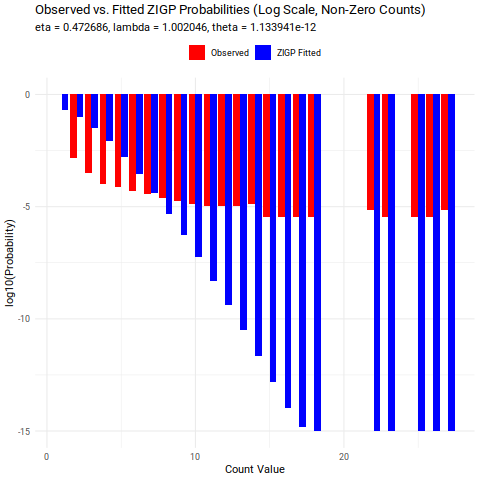
\includegraphics[totalheight=8cm]{plot_zigp_comparison_fixed.png}
    \caption{The observed and expected values. The 0 counts are not shown, and the missing bars are count values that
      were not observed.}
    \label{figure:plot_zigp_comparison_fixed.png} 
  \end{center}
\end{figure}

Then the marker pairs were ranked based on the count and only the pairs having count
more than 2 were retained. A threshold of at least two ($t = 2$) appearances as parent-child nodes in the decision trees
of the Random Forests was used because the use of one ($t = 1$) resulted in a substantially higher number of SNP pairs,
often random occurrences, that did not improve the identification of interactions.  Finally, using linear models the
significance of the interactions are tested. For a linear model, an interaction occurs when an independent variable has
a different effect on the outcome depending on the values of another independent variable. The variables in the model
are divided between main and interaction effects. A multiplicative epistasis model was used, where the interaction
between two markers, $i$ and $j$, are modelled as the product of the two genotype values, using the following linear
regression model:

\begin{equation}
  y = \beta_0 + \beta_i x_i +  \beta_j x_j + \beta_{i,j} x_ix_j + \epsilon.
  \label{eqn:linearmmodel}
\end{equation}

Here $y$ is the qualitative measure of phenotype, and $x$ are the genotype values \{0, 1, 2\}  for SNP $i$ and $j$ respectively,
$\beta_0$ is the mean phenotype, and  $\{\beta_i, \beta_j\}$ are the marginal effects for SNP $i$ and $j$, $\beta_{i,j}$
is the interaction effect between SNP $i$  and  $j$, and $\epsilon$ is the residual with $N(0,1)$. For case-control disease data, the interaction was modelled
through a logit function as follows:

\begin{equation}
  \logit (P(y =1)) =  \beta_0 + \beta_i x_i +  \beta_j x_j + \beta_{i,j} x_ix_j + \epsilon,
  \label{eqn:logitmodel}
\end{equation}
where '1' is the disease state and '0' is the control state.  An interaction is considered identified when the p-value of $\beta_{i,j}$ is significant.


\begin{figure}[thbp]
  \begin{center}
    \centering
    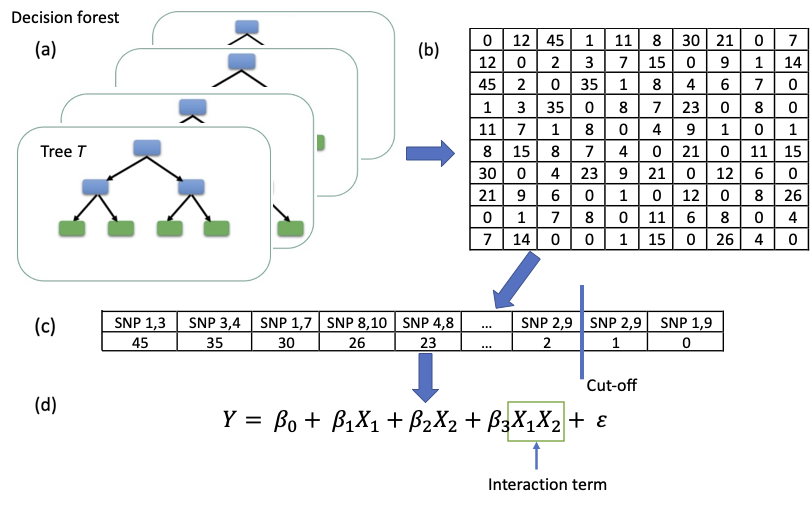
\includegraphics[totalheight=5cm]{Figure_1.png}
    \caption{The stages of the proposed method. (a) A Random Forests model is trained with all genomic markers. (b) A
      parent-child node count matrix is generated. (c) Marker pairs are ranked based on the number of appearances as
      parent-child pairs. (d) Using linear model, interaction tests are performed only for the selected marker pairs. }
    \label{figure:RF_Method} 
  \end{center}
\end{figure}

\subsection{Simulation data}

Three different interaction scenarios were considered to access the performance of the proposed method in detecting
pairwise interactions.  A simulated dataset was generated using publicly available genotype data containing of 3,534
animals from a single PIC nucleus pig line genotyped using the Illumina ProcineSNP60 chip \cite[]{clevelandCommonDatasetGenomic2012}. The
original dataset contained 52,843 single nucleotide polymorphisms (SNP) but in this study, all non-informative SNPs were
removed leaving 48,015 markers.  The simulated data was created by randomly selecting 5,000; 10,000 and 48,000 markers
from the dataset.  Using these three datasets, simulated phenotypes were then created having different heritabilities
$(h2 = 0.25, 0.33, 0.50, 0.66, 0.75 \textrm{ and } 1.00)$. Data was generated using three different models, a ``Base model'' where none
of the markers nor their interactions have any effect on the phenotype; a ``No Interaction model'' where markers have
marginal effects but there is no additional interaction effect, and an ``Interaction model'' where three pairs of markers have no marginal effects but have interaction
effects. The scenarios can be summarised as:
\begin{itemize}
\item  Base model phenotype = sum of ten QTL effects + noise (depending on heritability);
\item No Interaction model phenotype = sum of ten QTL effects + sum of marginal effect of epistatic SNPs (no interactions) + noise (depending on heritability);
\item  Interaction model phenotype = sum of ten QTL effects + sum of interaction effects for the three pairs (no   marginal effects) + noise (depending on heritability).
\end{itemize}


\subsection{Real datasets -- Wellcome Trust Case Control Consortium data for rheumatoid arthritis}
\label{subsection: rheumatoid}
The first dataset was obtained from the Wellcome Trust Case Control Consortium (WTCCC)
\cite[]{burtonGenomewideAssociationStudy2007brief}. The original dataset contains 14,000 cases for seven complex human
diseases and 3,000 shared controls. The control individuals were from two different sources: 1958 British Birth Cohort
(58C) and the UK Blood Service Control Group (UKBS). Each of the control group has 1,500 individuals. Samples of DNA
from all 17,000 individuals were genotyped with the GeneChip 500K Mapping Array Set (Affymetrix chip).  The current
analysis only used the data for rheumatoid arthritis (RA) that consisted of 4,798 individuals with 1,860 cases and 2,938
controls. Variants having $>10\%$ missing values and MAFs$<0.05$ were removed. SNP markers that failed the
Hardy-Weinberg test (p $\leq$ 0.05) were also removed. As linkage disequilibrium (LD) could affect how the Random Forests
(RF) algorithm selects a SNP at a particular node (for more detail how LD can affect RF, please see
\cite{mengPerformanceRandomForest2009}), the dataset was also filtered based on LD. Using PLINK 1.9
\cite[]{purcellPLINKToolSet2007} and a sliding window of 200 kb, one SNP from a pair of SNPs in that window was removed
if pairwise $r^2 >=0.3$.


\subsection{Real datasets -- Mouse data}
The second real data set we used was published by \cite{solbergProtocolHighthroughputPhenotyping2006};
\cite{valdarGeneticEnvironmentalEffects2006}. A curated version of this dataset was downloaded (Additional file 1 in
\cite{martiniGenomicPredictionEpistasis2017}). The curated mouse dataset contained 9,265 SNPs for each of 1,298
individuals. Pre-corrected residuals of thirteen phenotypes were available as phenotypes. In the current analysis, the
phenotype ``weight at six weeks'' (W6W) was used.



\section{Results and Discussion}
\subsection{Simulated data}
The method's performance was assessed by determining the number of interactions that were correctly identified and
through evaluating the repeatability and false discovery rate for the approach.  The evaluation of the method's ability
to correctly identify interacting markers was assessed based on the proportion of times, the method selected the
interacting marker pairs for pairwise interaction tests. Table  \ref{table:ranking10qtl} shows the importance ranking of three interacting SNP
pairs based on the number of times they appeared as parent-child nodes in the Random Forests decision trees. Higher
ranking, represented by a smaller number, meant a higher count.  For example, a value of 1 for pair P3 means that SNP
pair 3 appeared as parent-child nodes more than any other pair of markers in that Random Forests analysis.


As was expected in the ``Base model'', three pairs of interacting SNP do not appear as parent-child nodes in any decision
tree of the Random Forests. This reflected that these SNP did not have any marginal or interaction effects. In the ``No
interaction model'', the three interacting SNP pairs appeared as parent-child nodes in some of the scenarios. This is
expected as in the ``No Interaction model'' all the individual SNP have their own marginal effects while not
interacting. Hence, they were correctly selected at different nodes of the decision trees.  For the ``Interaction model'',
rankings of the three interacting SNP pairs are relatively higher than the other two models. The rankings observed
demonstrated that if the SNP pairs are ranked based on the count of their appearance as parent-child nodes, it should be
possible to only test pairwise interaction for a subset of marker pairs from the vast number of total possible combinations-
 of markers.  To quantify the efficiency of the method in reducing the search space, the number of tests performed
was compared to the number of markers and potential pairwise combinations. For this test, a threshold of $t = 2$ was
used, meaning that if any of the marker pairs appeared as parent-child nodes in the decision trees of the Random Forests
for at least twice, they were then tested for interaction significance using Equation \ref{eqn:linearmmodel}. Table  \ref{table:Number.of.tests.performed.to.detect.interactions} shows the number of
pair-wise interaction tests performed for the ``Interaction model'' alongside the number of possible pairwise combinations
for specified sets of heritability and marker numbers. The final column of Table  \ref{table:Number.of.tests.performed.to.detect.interactions} shows that for all scenarios, less
than one percentage of the total marker pairs were tested for interaction.  In all cases, including for the largest
simulated dataset with 48,000 markers, the three interacting pairs (P1, P2 and P3) were selected for pairwise
interaction tests.

Table  \ref{table:Number.of.tests.performed.to.detect.interactions} demonstrates that, as the number of markers increased the total number of tests performed decreased. This result
is due to the fact that the number of trees (num.tree = 1000) and a threshold of $t = 2$ remained the same for all
simulations. Thus, as combinatorial search space increases due to increasing numbers of markers, the number of pairs of
markers that exceed the parent-child node threshold ($t = 2$) is reduced. This suggests that for smaller marker sets,
the number of decision trees could be reduced to minimise computation and time demands. One strategy could be to
adjust the number of decision trees dependent on the number of markers.


  \begin{table}
\begin{center}
	\begin{tabular}{|p{0.7cm}|c|p{0.375cm}p{0.375cm}p{0.375cm}|p{0.375cm}p{0.375cm}p{0.375cm}|p{0.375cm}p{0.375cm}p{0.375cm}|}
 \hline
Num SNP  & H2     &   \multicolumn{3}{|c|}{Base Model}&    \multicolumn{3}{|c|}{No Interaction}  &
                                                                                               \multicolumn{3}{|c|}{Interaction}\\
          \hline
          &    & P1 & P2 & P3 & P1   & P2  & P3   & P1  & P2 & P3 \\
          \hline
\parbox[t]{2mm}{\multirow{3}{*}{\rotatebox[origin=c]{90}{5,000}}}  & 0.33 & NC & NC & NC & 323  & 2   & 287  & 10  & 5  & 7  \\
         & 0.50 & NC & NC & NC & 151  & 1   & 3373 & 6   & 4  & 10 \\
         & 0.66 & NC & NC & NC & 730  & 3   & 699  & 8   & 4  & 9  \\
          & 1.00 & NC & NC & NC & 230  & 1   & 315  & 7   & 3  & 11 \\
          \hline
\parbox[t]{2mm}{\multirow{3}{*}{\rotatebox[origin=c]{90}{10,000}}}  & 0.33 & NC & NC & NC & NC   & 20  & NC   & 132 & 9  & 3  \\
         & 0.50 & NC & NC & NC & NC   & 40  & NC   & 293 & 7  & 1  \\
         & 0.66 & NC & NC & NC & NC   & 59  & NC   & 88  & 5  & 1  \\
          & 1.00 & NC & NC & NC & 1077 & 32  & NC   & 86  & 6  & 1  \\
          \hline
\parbox[t]{2mm}{\multirow{3}{*}{\rotatebox[origin=c]{90}{48,000}}}  & 0.33 & NC & NC & NC & NC   & NC  & NC   & 4   & 50 & 63 \\
         & 0.50 & NC & NC & NC & 204  & 412 & NC   & 5   & 27 & 12 \\
         & 0.66 & NC & NC & NC & 806  & 224 & NC   & 2   & 30 & 13 \\
          & 1.00 & NC & NC & NC & 663  & 118 & 909  & 13  & 45 & 9  \\
          \hline
\end{tabular}
\end{center}
\caption{Ranking of the SNP pairs based on counts. Simulated data for 10 QTL and 3 pairs of interactions.
  NC = No count. P1, P2 and P3 are three interacting SNP pairs.}
\label{table:ranking10qtl}
\end{table}


\begin{table}
\begin{center}
	\begin{tabular}{|c|c|p{1.6cm}|p{1.6cm}|p{1.6cm}|}
 \hline
          Num SNP & H2   & Num test performed & Num of possible combination & Percentage  \\
          \hline
5,000             & 0.33 & 61,346             & 12,497,50                   & 0.004909        \\
                  & 0.50 & 62,610             & 12,497,50                   & 0.00501         \\
                  & 0.66 & 64,111             & 12,497,50                   & 0.00513         \\
                  & 1.00 & 57,747             & 12,497,50                   & 0.004621        \\
      \hline
10,000            & 0.33 & 18226              & 49,995,00                   & 0.000365        \\
                  & 0.50 & 18938              & 49,995,00                   & 0.000379        \\
                  & 0.66 & 20324              & 49,995,00                   & 0.000407        \\
                  & 1.00 & 21204              & 49,995,00                   & 0.000424        \\
       \hline
48,000            & 0.33 & 1742               & 1.15E+09                    & 1.51E-06        \\
                  & 0.50 & 2400               & 1.15E+09                    & 2.08E-06        \\
                  & 0.66 & 3064               & 1.15E+09                    & 2.66E-06        \\
                  & 1.00 & 5531               & 1.15E+09                    & 4.80E-06        \\
        \hline
\end{tabular}
\end{center}
\caption{Number of tests performed to detect interactions.}
\label{table:Number.of.tests.performed.to.detect.interactions}
\end{table}


\subsection{Heritability}

The effect of heritability on the method's performance was explored with the pairwise counts for each of the
interacting SNP pairs in each Random Forests at different heritabilities (h2 = 0.33, 0.50, 0.66, and 1.00) for 10,000
SNP with 10 QTL and 3 pairs of interacting SNPs recorded. The results are shown in Figure \ref{figure:Eff_Trait_h2_simulated_data.png}. At lower heritabilities,
the pairwise count is small and as heritability increases, the pairwise count also increases. Although the three
interacting SNP pairs have very similar interaction effects (ranging between 0.3 to 0.4), they have very different
numbers of counts. There is a direct relationship between the $p$-value of the interaction term with the pairwise
count. Lower $p$-values of the interaction terms have higher pairwise count (correlation coefficient = 0.84, $p$-values
and correlations are not shown). This is particularly interesting as even very small interaction effects with high
significance will not be overlooked because of higher pairwise count.



\begin{figure}[thbp]
    \begin{center}
  \centering
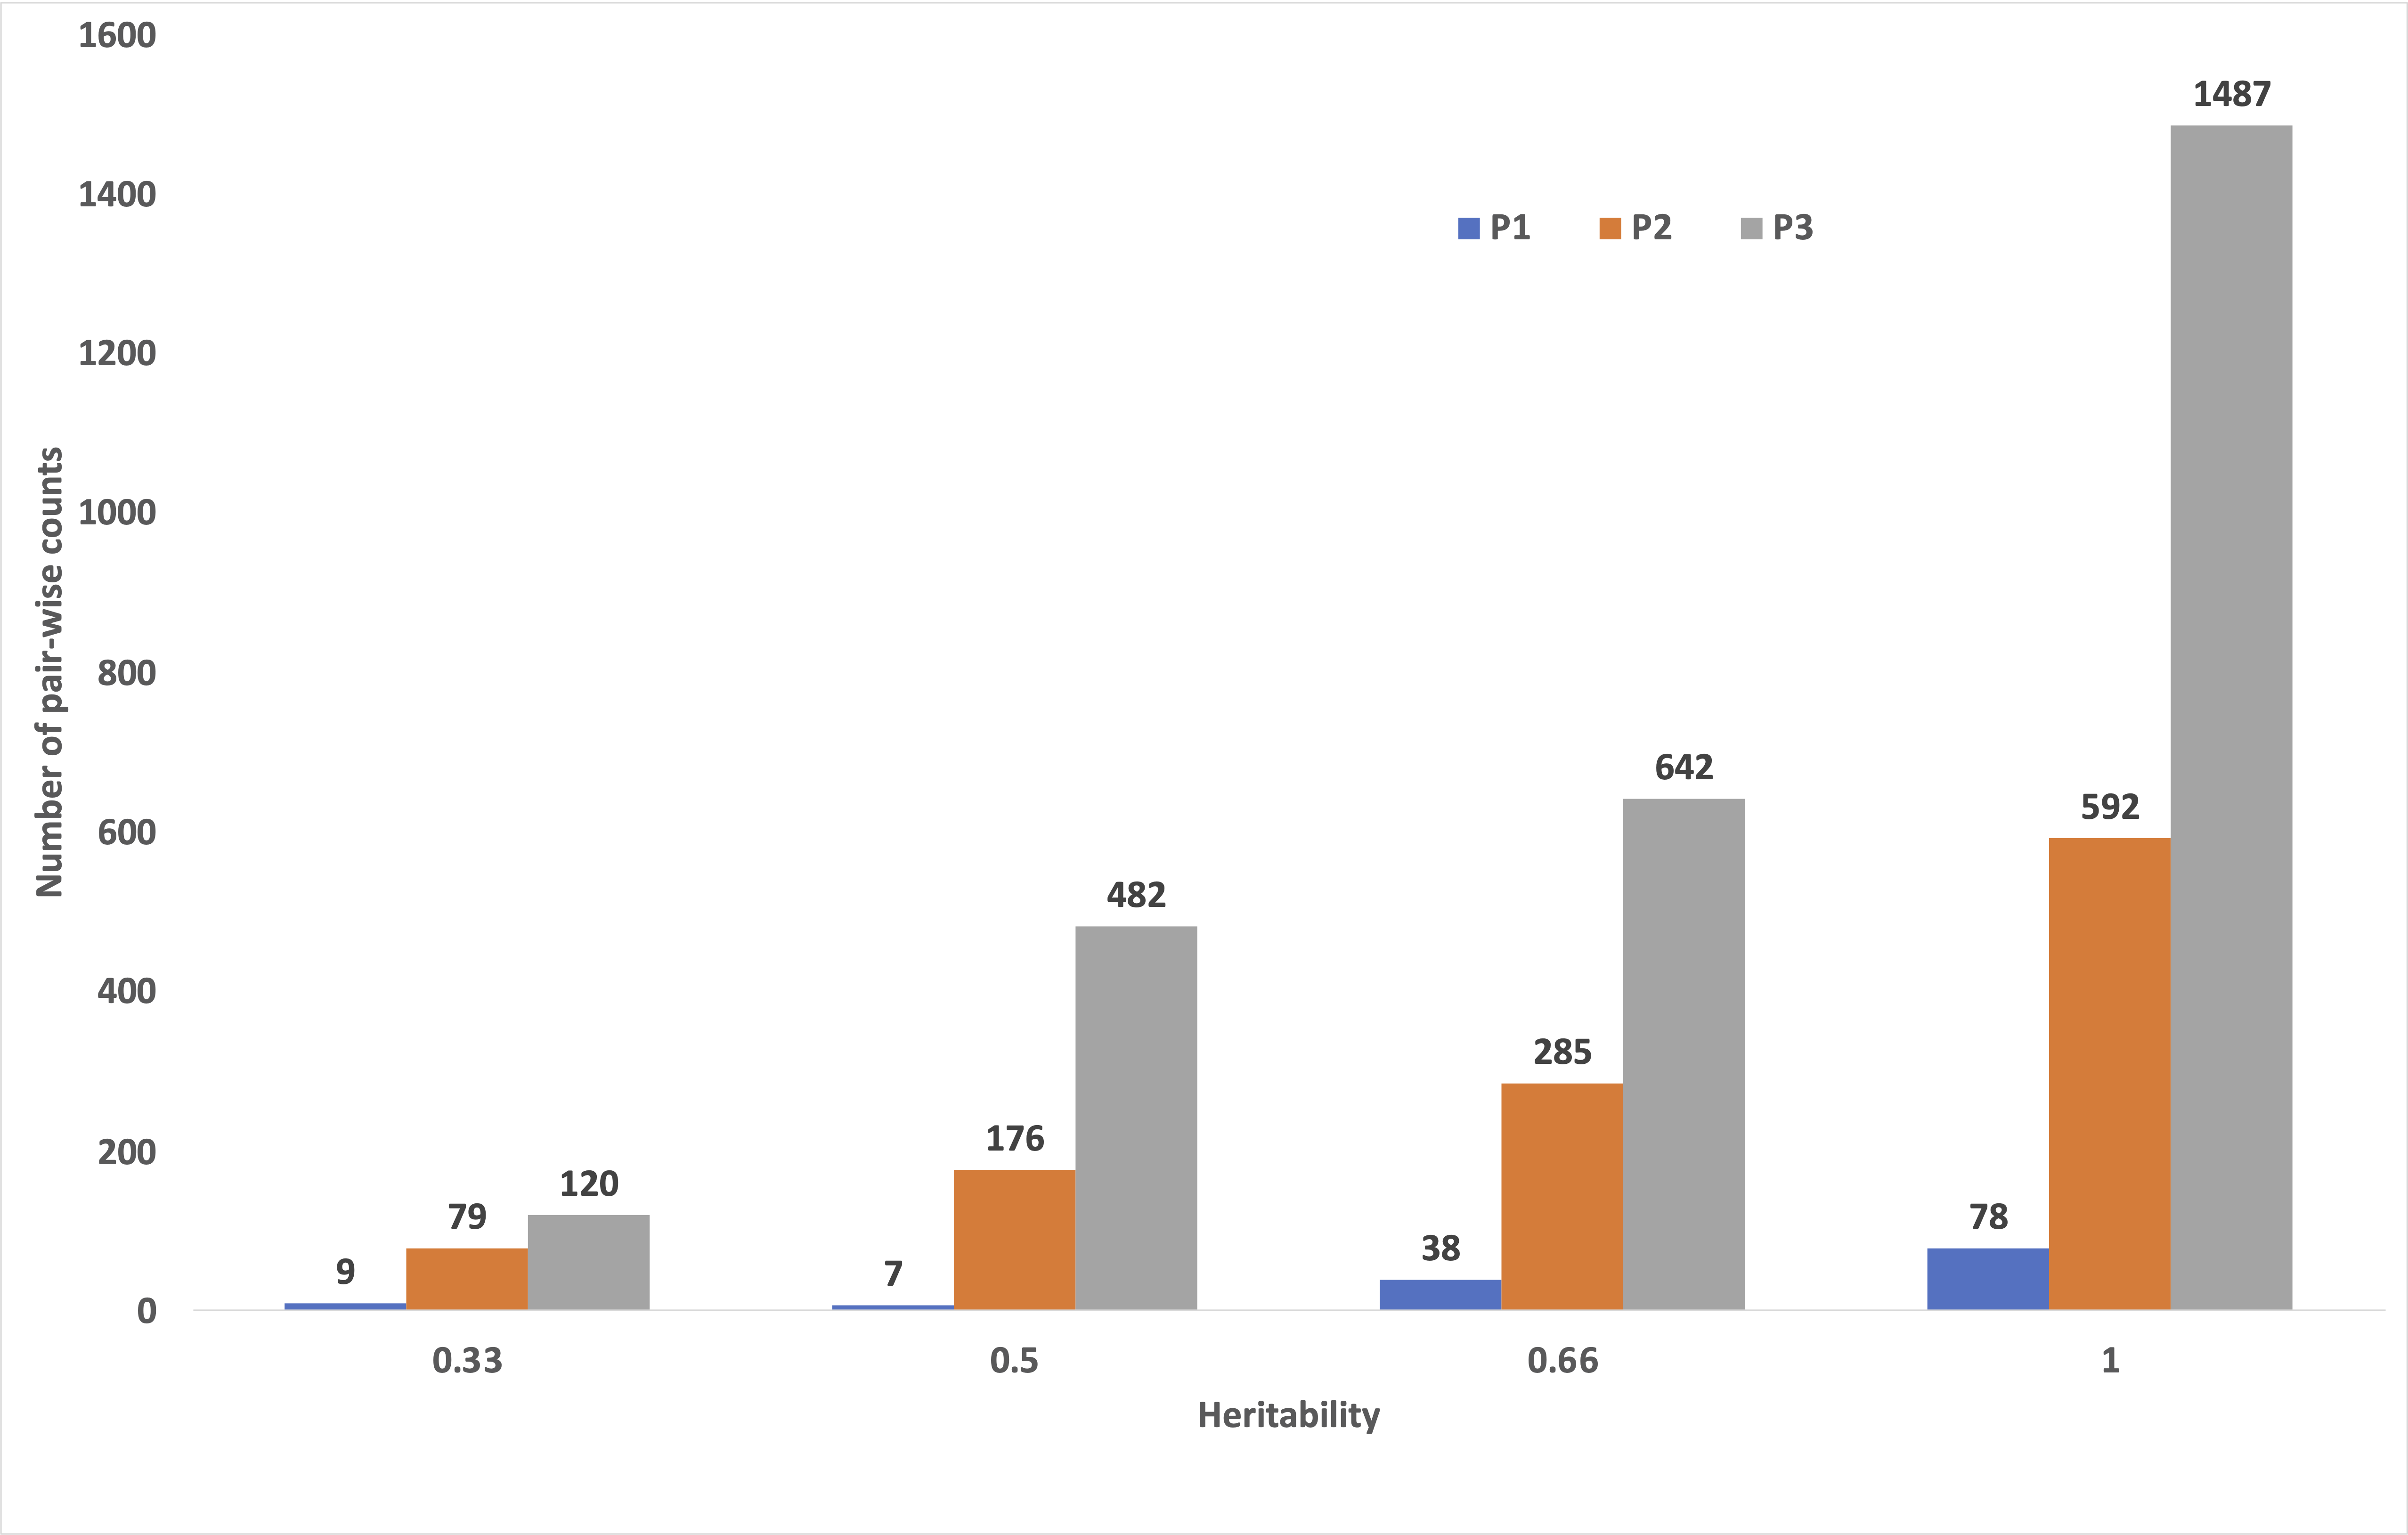
\includegraphics[totalheight=5cm]{Figure_2.png}
\caption{ The effect of trait heritability on pairwise counts. P1, P2 and P3 are interacting SNP pair 1, 2 and 3 respectively.
The Y- axis shows the number of pairwise counts for each interacting SNP pair in each Random Forests.}
  \label{figure:Eff_Trait_h2_simulated_data.png} 
    \end{center}
\end{figure}


\subsection{Repeatability and false discovery rate}

To test repeatability of the proposed method, the ``Interaction model'' was generated ten times at each heritability
(0.25, 0.33, 0.50, 0.66, and 0.75) with the correct identification of the interacting marker pairs assessed. Table
\ref{table:Repeatability_of_the_proposed_method} shows the results for 10,000 SNPs with 10 QTLs and 3 pairs of
interacting SNPs. In most of the scenarios tested, the method was able to successfully identify the interacting pairs
except for pair P1 at lower heritabilities. This result appears to be because pair P1 has a lower interaction effect
when compared to pairs P2 and P3. Pair P1 appeared on the candidate lists in all instances but did not pass multiple
test corrections several times when the heritabilities were low (i.e. 0.25, 0.33).  To assess the false discovery rate of
the method, the number of false positive interactions were counted across the 10 replicates at the different
heritability levels. A false positive was declared when a pair of SNP were not in the original data and when these SNP
were not correlated or in high LD with one of the three simulated pairs. This is because there were multiple
interactions identified where each marker in the pair correlated highly with corresponding markers in one of the
simulated interaction pairs.  Only when this was not the case was a false positive declared. A Pearson correlation
coefficient of less than 0.25 was used as the threshold. This threshold was chosen as using a 0.5 threshold revealed a
number of pairs incorrectly identified as false positives where each marker in the pair was correlated, normally with a
coefficient above 0.4, with one of the simulated three pairs. The mean false positive results for each heritability
calculated using the ten replicates, are shown in Table \ref{table:Repeatability_of_the_proposed_method}. The number of
false positives increased in the data where the heritability was higher. This was understandable as the variance
explained by the marker data (genetic signal) increases at higher heritabilities.

The number of false positives detected by the proposed method was low across all heritabilities.


\begin{table}
  \begin{center}
    \begin{tabular}{|ccccc|}
      \hline
      $h^2$ & P1 & P2 & P3   &  False + \\
      \hline                
      0.75  & 10 & 10 & 10   &  0\\
      0.66  & 10 & 10 & 10   &  0.1 \\
      0.50  & 9  & 10 & 10   &  0.3 \\
      0.33  & 7  & 10 & 10   &  0.8 \\
      0.25  & 4  & 10 & 10   &  1.9 \\
      \hline          
    \end{tabular}
  \end{center}
  \caption{Repeatability and number of false positives for the proposed method. The data contains 10,000 with 10 QTLS and 3 pairs of interacting SNP.
    The process was repeated 10 times for each heritability with the number of times each pair (P1, P2 or P3) found and the mean number of false positive
    interactions identified indicated.}
  \label{table:Repeatability_of_the_proposed_method}
\end{table}



\section{Results for real datasets}
To evaluate the method's performance on real data, two real datasets were assessed for the presence of interacting SNP
pairs.


\subsubsection{Rheumatoid arthritis data}
After pre-processing and filtering, the Rheumatoid arthritis (RA) dataset contained 94,486 SNPs (4.46 billion possible
pairwise interaction tests) and 4,798 individuals. The method, after building a Random Forests analysis, selected only
654 SNP pairs for the second stage of testing to identify significant pairwise interactions (Equation \ref{eqn:logitmodel}). Among the
654 SNP pairs, 26 pairs were found significant using a Bonferroni corrected $p$-value ($p < 0.05$). Specifically, a total of
24 SNP were involved in 26 significant interactions among which 22 of these SNP were from chromosome 6 with two
markers from chromosome 1 and chromosome 7. Furthermore, several SNPs from chromosome 6 were involved in multiple
interactions. All 22 SNP on chromosome 6 were located in the HLA (human leukocyte antigen) region spanning from 31.35 MB
to 32.80 MB. The HLA region in the human genome is known to be highly conserved with high linkage disequilibrium
between markers in the region. If interacting SNP pairs are in the same haplotype or LD block, the significant
interaction between the pairs might be a result of a haplotype effect on RA, rather than true interaction. Out of the 26
pairs of interacting SNPs, 12 pairs (all markers on chromosome 6) have moderate to high LD (D' = (0.26 to 0.55)) between
the pairs.  These were deemed to likely be significant due to being part of the same haplotype. Thus, only 14 SNP pairs
with low LD (D' $\leq$ 0.2) were retained for further investigation.

Table \ref{table:eight.pairs} lists the 14 interacting SNP pairs that were found using the method to be associated with rheumatoid arthritis
in humans.  Genes containing any of the interacting SNPs as well as flanking genes for intergenic SNP are listed in
Supplementary Table S1.


All 14 significant SNP pair interactions had at least one SNP of each pair positioned in the
major histocompatibility complex (MHC) class II centred on the HLA-DQ to HLA-DR regions located in chromosome 6p21. The
HLA region in human chromosome is a 3.78 Mb region that is the most gene dense region within the human genome,
encoding about 253 genes including several key immune response genes \cite[]{shiinaHLAGenomicLoci2009a}. The genes in this region
predominantly have immune response functions. The dominance of the HLA-DQ to HLA-DR region in the interacting SNPs may
be due to several factors including the clustering of genes with key roles in immune response and its regulation, high
gene density including some overlapping and anti-sense genes, and a high rate of polymorphism and therefore high linkage
disequilibrium.  The identification of 12 pairs with both SNP in the HLA-DQ - HLA-DR region on chromosome 6p21
demonstrates that the proposed method is able to identify cis-acting positive and negative SNP interactions
identifying potential gene interactions in this gene-dense HLA-DQ - HLA-DR region.  The identified SNPs may be genetic
markers closely linked to causal genetic variants or it is also possible that some of the interacting SNPs may be
causal. Two identified interacting pairs of SNP (rs615672/rs9268831 and rs92688831/rs615672) were found to have both
markers in potential genome regulatory elements. Collectively, this information suggests that local gene-gene
interactions in this region could be mediated by cis-acting regulatory mechanisms involving short and long range DNA
loops. Some of the identified interactive SNPs were located near or within introns of genes unrelated to the HLA-DQ and
HLA-DR
genes but interspersed within the same region on chromosome 6p21. These genes included NOTCH4 (notch receptor 4),
TNXB (tenascin XB) and BTNL2 (butryophilin-like 2). NOTCH4
regulates cell fate determination, proliferation and apoptosis
programs and has a regulatory role in branching morphogenesis
in the developing vascular system. It is also implicated in the
regulation of inflammation
\cite[]{harbRegulatoryCellNotch4GDF152020,zhengNotch4NegativelyRegulates2018}
, a characteristic feature of autoimmune diseases such as
rheumatoid arthritis. TNXB encodes a tenascin family member of
extracellular matrix proteins. It has anti-adhesive effects and is
involved in extracellular matrix maturation following wound
healing \cite[]{stelzerGeneCardsSuiteGene2016}
. Thus, the protein encoded by
TNXB may potentially be involved in tissue repair after damage
caused by chronic inflammation. BTNL2 belongs to a family of
immune regulators. It decreases T-cell proliferation and cytokine
release during an inflammatory response and has been implicated in a number of autoimmune diseases
\cite[]{arnettBTNL2ButyrophilinB7Like2007,stelzerGeneCardsSuiteGene2016,lebrero-fernandezAlteredExpressionButyrophilin2016a}.


The SNP interaction partner to the SNP identified in BTNL2 on 6p21 is located near NRF1 (nuclear respiratory facto 1) on
chromosome 7. NRF1 encodes a transcription factor activating key metabolic and cell growth genes as well as
mitochondrial DNA transcription and replication. NRF1 has also been implicated in the regulation of inflammation
\cite[]{stelzerGeneCardsSuiteGene2016,vantienenProlongedNrf1Overexpression2010, yangNglycanaseNGLY1Regulates2018}.


One possibility is that NRF1 acts in trans directly or indirectly via its encoded transcription factor to regulate BTNL2
expression on chromosome 6p21 and thus modulate T-cell mediated immune activation and inflammation.

Notably, multiple genome wide association studies (GWAS) identified a subset of the interactive SNPs as associated with
various autoimmune diseases i.e., rs9273363, rheumatoid arthritis; type 1 diabetes; rs6457617, multiple sclerosis,
Graves disease, systemic sclerosis; rs615672, rheumatoid arthritis \cite[]{UCSC.2022}.
The results fromusing the proposed method on the human rheumatoid arthritis data revealed a number of promising results supporting the
potential value of the proposed method for identifying epistatic interactions in case control data including the
ability to find positive and negative cis-acting interactions.

The results from using the proposed method on the human rheumatoid arthritis data revealed a number of promising results
supporting the potential value of the proposed method for identifying epistatic interactions in case control data
including the ability to find positive and negative cis-acting interactions.


\begin{sidewaystable}
  \tiny
 \begin{center}
   \begin{tabularx}{\textwidth}{|c|c|c|p{1.16cm}|p{0.8cm}|p{1.16cm}|c|c|p{0.8cm} |c|c|c|c|p{1cm}||}
 \hline
 SNP pair & D' & r$^2$ & 
      \rotatebox{60}{SNP1 location} & 
      \rotatebox{60}{\makecell{SNP1 odds\\ ratio}} & 
      \rotatebox{60}{\makecell{SNP1 odds ratio \\(95\% CI)\textsuperscript{b}}} &
      \rotatebox{60}{SNP1 $p$-value\textsuperscript{d}} & 
      \rotatebox{60}{SNP2 location} & 
      \rotatebox{60}{\makecell{SNP2 odds\\ ratio}} & 
      \rotatebox{60}{\makecell{SNP2 odds ratio \\ (95\% CI)\textsuperscript{b}}} &
      \rotatebox{60}{SNP2 $p$-value\textsuperscript{d}} & 
      \rotatebox{60}{\makecell{Interaction \\Odds ratio}} &
      \rotatebox{60}{\makecell{Interaction Odds ratio\\ (95\% CI)\textsuperscript{c}}} & 
      \rotatebox{60}{\makecell{Interaction\\ $p$-value\textsuperscript{d}}} \\
      \hline
   rs3134926:rs910050     & 0.10 & 0.01 & 6:32232370  & 0.61 & 0.55,0.6  & 1.99E-20 & 6:32347877 & 0.79 & 0.72,0.86 &  7.11E-05& 1.77 & 1.53,2.06 & 3.38E-11 \\
 rs3134926:rs4530903      & 0.14 & 0.01 & 6:32232370  & 0.61 & 0.55,0.67 & 1.99E-20 & 6:32614112 & 1.41 & 1.24,1.59 &  6.59E-05& 1.64 & 1.34,2.01 & 9.90E-04 \\
 rs9431614:rs9296009      & 0.01 & 0.00 & 1:230944623 & 1.00 & 0.89,1.11 & 5.17E+02 & 6:32146738 & 1.80 & 1.64,1.97 &  2.51E-33& 1.62 & 1.35,1.96 & 2.91E-04 \\
 rs3134926:rs9391858      & 0.06 & 0.00 & 6:32232370  & 0.61 & 0.55,0.67 & 1.99E-20 & 6:32373621 & 1.24 & 1.11,1.39 &  5.76E-02& 1.55 & 1.28,1.88 & 4.22E-03 \\
 rs10456058:rs9273363$^a$ & 0.08 & 0.00 & 6:31526961  & 1.11 & 1.03,1.21 & 5.97   & 6:32658495 & 1.34 & 1.23,1.46 &  3.39E-08& 1.50 & 1.32,1.7  & 2.73E-07 \\
 rs910050:rs6457617       & 0.17 & 0.02 & 6:32347877  & 0.79 & 0.72,0.86 & 7.11E-05 & 6:32696074 & 0.44 & 0.4,0.48  &  1.06E-69& 1.39 & 1.22,1.59 & 4.32E-04 \\
 rs9268831:rs615672       & 0.15 & 0.01 & 6:32459971  & 0.69 & 0.63,0.75 & 3.37E-16 & 6:32606394 & 0.60 & 0.54,0.66 &  7.78E-24& 1.34 & 1.17,1.53 & 9.12E-03 \\
 rs2076533:rs1270689      & 0.03 & 0.00 & 6:32395750  & 0.49 & 0.45,0.54 & 4.60E-55 & 7:12961515 & 1.06 & 0.98,1.16 &  8.23E+1& 1.31 & 1.16,1.48 & 1.48E-02 \\
 rs17421624:rs615672      & 0.18 & 0.01 & 6:32098400  & 1.70 & 1.56,1.86 & 7.24E-31 & 6:32606394 & 0.60 & 0.54,0.66 &  7.78E-24& 0.73 & 0.64,0.84 & 7.58E-03 \\
 rs6457617:rs2621382$^e$      & 0.17 & 0.03 & 6:32696074  & 0.44 & 0.4,0.48  & 1.06E-69 & 6:32792668 & 1.02 & 0.94,1.11 &  3.44E+02& 0.73 & 0.64,0.83 & 6.46E-04 \\
 rs17421624:rs3134926     & 0.08 & 0.00 & 6:32098400  & 1.70 & 1.56,1.86 & 7.24E-31 & 6:32232370 & 0.61 & 0.55,0.67 &  1.99E-20& 0.72 & 0.62,0.83 & 7.12E-03 \\
 rs17421624:rs427037      & 0.03 & 0.00 & 6:32098400  & 1.70 & 1.56,1.86 & 7.24E-31 & 6:3224448  & 0.70 & 0.62,0.78 &  2.70E-07& 0.69 & 0.59,0.82 & 1.11E-03  \\
rs9296009:rs4530903       & 0.10 & 0.00 & 6:32146738  & 1.80 & 1.64,1.97 & 2.51E-33 & 6:3261411  & 1.41 & 1.24,1.59 &  6.59E-05& 0.67 & 0.55,0.81 & 3.16E-03  \\
rs206015:rs3134926        & 0.06 & 0.00 & 6:32214982  & 1.49 & 1.33,1.67 & 2.90E-09 & 6:32232370 & 0.61 & 0.55,0.67 &  1.99E-20& 0.67 & 0.55,0.82 & 4.66E-03  \\
\hline
\end{tabularx}
% \end{tabular}
 \end{center}
 \caption{Eight pairs of interacting SNPs have significant odds ratio after pairwise LD evaluation}
 \label{table:eight.pairs}
 \begin{tablenotes}%
 \item $^{a}$ rs10456058 has merged into rs2734573.
 \item $^{b}$  Odds ratio (OR) of having at least one copy of the risk allele compared to having 0 copies of the same allele for the given SNP.
 \item $^{c}$  Odds ratio (OR) of having at least one copy of each risk allele compared to having 0 copies of the same allele for the given SNP pair.
 \item $^{d}$  Bonferroni adjusted p-value.
 \item $^e$   The pair of SNPs used as an example in section \label{section:A_linear_model_example}.
 \end{tablenotes}
\end{sidewaystable}

\subsection{Mouse  data}
The curated mouse data contained 9,265 SNPs resulting in nearly 43 million possible pairwise comparisons to test for the
presence of significant interactions contributing to the phenotype ``weight at 6 weeks''. The proposed method, identified
273,391 pairs of SNP (0.0064\%) for the second stage of interaction testing. After using the Bonferroni multiple testing
correction, 59 pairs of interacting SNPs remained as significant. These 59 pairs of interactions were from 63 unique
SNPs mainly located on MMU chromosomes 2, 8 and 13. To check the validity of the results and proposed method, the genes
associated with each of these SNP were identified using the Mouse Genome Informatics \cite[]{mgi}.

Supplementary Table S2  lists the significant interacting pairs of SNPs that were found associated with the
murine growth trait W6W. The nearest genes (mean distance = 36.7 Kbp; range = 42 bp - 286 Kbp) associated with these SNP
are also listed. The associated MGI ID (Mouse Genome Informatics ID), Entrez ID and GO terms (Gene Ontology) are listed
in Supplementary Table S3. 
The proposed method identified four genes and two functionally
anonymous genes (miR8108 and Gm31784) associated with two additional SNPs, in a 3.8 Mbp interval on MMU Chr8qA2.  Genes
Tm2d2, Tacc1, Slc20a2 and Fgfr1 are contained within a small region of 0.5 Mbp of this larger segment and have a variety
of functions that potentially impact a phenotype associated with growth and development. Fgfr1 (fibroblast growth factor
receptor 1) has wide ranging biological functions associated with regulation of cell division, cell growth and
maturation, embryonic development, wound healing, and formation of blood vessels. In humans, the cellular signalling
mediated by this receptor has roles in the development and growth of bones, particularly bones in the head, face, hand,
feet, and long bones of the arms and legs. Mutations in the gene are associated with human dwarfism (National Institutes
of Health, 2021). Tacc1 (transforming acidic coiled-coil containing protein 1) is involved in processes that promote
cell division before the formation of differentiated tissues \cite[]{stelzerGeneCardsSuiteGene2016}. Tacc1 encodes a protein that
regulates the localization of nuclear receptors, including T3 thyroid hormone and retinoic pathways involved in regula-
tion cell growth and differentiation. Tm2d2 (TM2 domain containing 2) encodes a G-coupled receptor that regulates cell
death and proliferation cascades \cite[]{stelzerGeneCardsSuiteGene2016}. Slc20a2 (solute carrier family 20 member 2) encodes an
inorganic phosphate transporter important in maintaining phosphate homeostasis.  This function is essential for all
intracellular function. The encoded protein also has roles in extracellular matrix and cartilage calcification, which
is important for tissue function \cite[]{stelzerGeneCardsSuiteGene2016}. It is noted that growing bones have high demands for phosphate
(Goretti Penido and Alon 2012).  Four genes identified as potentially involved in interactions were located in a 0.25
Mbp region on the MMU Chr2qA3- 2qB boundary. They were (Mrps2 (mammalian mitochondrial ribosomal protein), Ralgds (ral
guanine nucleotide dissociation stimulator), Ddx31 (dead-box helicase 31) and Ttf1 (transcription termination factor
1). These genes have a variety of functions including mitochondrial protein synthesis, intracellular signalling, cell growth and division in embryogenesis, and
transcription, respectively \cite[]{stelzerGeneCardsSuiteGene2016}. At present, only Ddx31 is directly linked to
growth related traits, although the molecular functions of the remaining three genes may have this potential.  The
remaining genes identified from the analyses, listed in Tables S2 and S3, map to various chromosomal regions. Notable
gene functions or mutational effects that could influence growth traits include: regulation of cell proliferation,
differentiation and survival (Klf7, Kruppel like factor 7); osteogenesis (Stmn2, Stathmin 2); short stature and skeletal
abnormalities (Wipi2, WD40 repeat protein interacting with phosphoinositides 2); increased blood testosterone,
precocious sexual maturation, increased fecundity, and clearance of luteinizing hormone (Chst8, carbohydrate
sulfo-transferase 8) \cite[]{stelzerGeneCardsSuiteGene2016}. In all, there were several genes identified close to
interacting SNPs listed in Tables S2 and S3 that have effects on murine growth and developmental traits, particularly
osteogenesis and body stature.  Analysis of the mouse data results revealed strong gene candidates for involvement in
growth and development pathways in mice, including genes known to have relevant biological function as well as novel
candidates. This finding indicates that the function of these genes could be influenced by interactions with other genes
and that the proposed method is able to identify multiple promising regions for a quantitative trait for further
exploration.



\section{Conclusion}

In this study, a novel efficient method to identify potentially interacting pairs of markers in genomic data for a
specific trait was proposed and validated. A Random Forests decision tree algorithm was utilised to select a subset of
markers pairs from, the often, vast search space to enable the efficient computational testing of these pairs for
evidence of significant interaction. The method was validated with several simulation datasets representing different
data structures and characteristics including marker density and trait heritability. The method was then used with two
real data sets to identify SNP interactions for two different type of traits, case-control data for the presence of
rheumatoid arthritis in humans, and quantitative trait data for the body weight of mice. In both cases, the method
identified several functionally relevant genes positioned close to the markers shown to be potentially interacting for
the respective traits. The method is demonstrated as having potential in providing new insights into the genetic basis
of complex traits controlled by multiple genes and their interactions. The method can be extended in a biological
context beyond purely genomic data to other 'omic data types or interactions between diverse types of data such as
marker and environmental data to further provide biological insights.


Key points:
\begin{itemize}
\item Detecting epistatic interactions from high dimensional genomic data is very challenging due to the computational
  burden induced by the large number of required combinatorial test.
\item Using a Random Forests algorithm, we provided a computationally simple way to detect pairwise interactions.
\item The method produced reliable results in the case of simulated and interpretable results in several real-world
  data sets.
\end{itemize}



%%%%%%%%%%%%%%
\appendix

\section{Data availability}
PIC nucleus pig line genotype data is available as supporting information in Cleveland et al., 2012. WTCCC genotype data
is available by application to the Wellcome Trust Case Control Consortium Data Access Committee. The mouse dataset is
available as Additional file 1 in \cite{martiniGenomicPredictionEpistasis2017}.


\FloatBarrier
\section{Competing interests}
There is NO Competing Interest.

\section{Author contributions statement}
H.A., R.D and K.V. conceived the experiment(s), H.A. conducted
the experiment(s), H.A., R.D. and R.T. analysed the results.  H.A., R.D and K.V. and R.T.  wrote and reviewed the manuscript.

\section{Acknowledgements}
This work is supported by CSIRO MLAI Future
Science Platform. This study makes use of data generated by the Wellcome Trust Case Control Consortium. A full list of
the investigators who contributed to the generation of the data is available from www.wtccc.org.uk. Funding for the
project was provided by the Wellcome Trust under award 076113.




%USE THE BELOW OPTIONS IN CASE YOU NEED AUTHOR YEAR FORMAT.
%\bibliographystyle{abbrvnat}
%\bibliography{reference}


\bibliographystyle{elsarticle-num}
\bibliography{./epistatic_interactions.bib}



\end{document}



